\documentclass[a4paper,11pt,eval]{nsi} 

\usepackage{pifont}
\usepackage{fontawesome5}
%\pagestyle{empty}


\newcounter{exoNum}
\setcounter{exoNum}{0}
%
\newcommand{\exo}[1]
{
	\addtocounter{exoNum}{1}
	{\titlefont\color{UGLiBlue}\Large Exercice\ \theexoNum\ \normalsize{#1}}\smallskip	
}



\begin{document}



\textcolor{UGLiBlue}{Vendredi 18/10/2024}\\
\classe{\premiere spé}
\titre{Evaluation Second degré - Sujet B}
\maketitle
\begin{center}
	Calculatrice interdite
\end{center}

%\vspace{.5cm}
\exo{}\bareme{5 pts}\\
On considère la fonction $f$ définie sur $\R$ par $\quad f(x)=\dfrac{1}{2}(x+2)^2-3$.

\begin{enumerate}%[label=\textbullet]
	\item 	Compléter le tableau de variation de $f$ sur $\R$ :
	\begin{center}
		\begin{tikzpicture}
			\tkzTabInit[lgt=3.5,espcl=3]
			{$x$ /.7 ,Variations de $f$ /2.5}
			{$-\infty$,,$+\infty$}
			\tkzTabVar{,,}
		\end{tikzpicture}
	\end{center}
	\item 	Calculer $f(0)$ et $f(2)$.\\[.5em]
	\carreauxseyes{16}{4}
	\item 	
	\begin{minipage}{7.7cm}
		Tracer la courbe représentative de $f$ dans le repère ci-contre.\\
        Indiquer les points utilisés.
	\end{minipage}
	\begin{minipage}{8.7cm}
		\begin{center}
			\def\xmin{-7} \def\ymin{-5}\def\xmax{6}\def\ymax{7}
			\begin{tikzpicture}[scale=.6]
				\clip (\xmin,\ymin) rectangle (\xmax,\ymax);
				\draw[fill = white] (\xmin,\ymin) rectangle (\xmax,\ymax);
				\repereal{\xmin}{\ymin}{\xmax}{\ymax}		
			\end{tikzpicture}
		\end{center}
	\end{minipage}
	
\end{enumerate}


\exo{}\bareme{7 pts}
\begin{enumerate}
    \item On définit la fonction $f$ sur $\R$ par $\quad f(x)=-2(x-3)^2+10$.
    \begin{enumalph}
        \item Donner la forme développée de $f$.
        \item Tracer l'allure de la courbe représentative de $f$ en précisant les points remarquables.
    \end{enumalph}
    \carreauxseyes{16}{9.6}
    \item On définit la fonction $g$ sur $\R$ par $\quad g(x)=\dfrac{1}{2}(x+2)(x-3)$.
    \begin{enumalph}
        \item Donner la forme développée de $g$.
        \item Tracer l'allure de la courbe représentative de $g$ en précisant les points remarquables.
    \end{enumalph}
    \carreauxseyes{16}{9.6}
\end{enumerate}

\exo{}\bareme{8 pts}\\
\begin{minipage}{9cm}
	Voici un carré de côté 8 auquel on a ôté deux carrés de côtés $x+1$ et $x+3$ \textbf{qui ne se chevauchent pas} pour 
	obtenir la forme dessinée
	en gris foncé.
\end{minipage}
\begin{minipage}{8cm}
	\begin{center}
		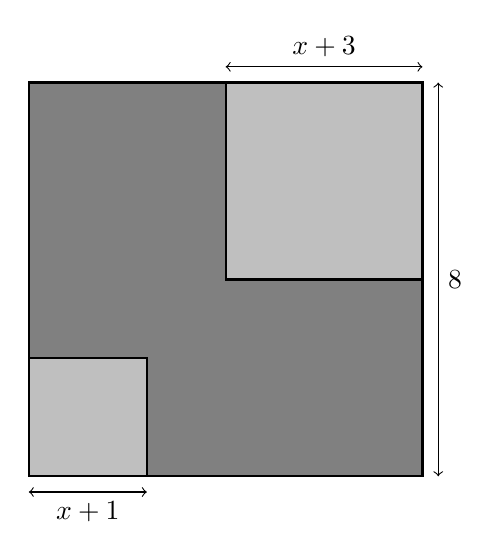
\begin{tikzpicture}[scale = .5]
			\draw[thick, fill = gray] (0,0)  rectangle (10,10);
			\draw[thick, fill = lightgray] (0,0)  rectangle (3,3);
			\draw[thick, fill = lightgray] (10,10)  rectangle (5,5);
			\draw[<->] (5,10.4) -- node[midway,above]{$x+3$} (10,10.4);
			\draw[<->] (10.4,0) -- node[midway,right]{8} (10.4,10);
			\draw[<->] (0,-.4) -- node[midway,below]{$x+1$} (3,-.4);
		\end{tikzpicture}
	\end{center}
\end{minipage}



\begin{enumerate}
	\item 	Quelle est la valeur minimale que peut prendre la variable $x$ ? Sa valeur maximale ?\\
    En déduire l'intervalle dans lequel varie $x$.\bareme{2 pts}\\[.5em]
	\carreauxseyes{16}{8}
	
	\item 	Montrer que l'aire $A(x)$ de la figure gris foncé est : $A(x)=-2x^2-8x+54$.\bareme{2 pts}\\[.5em]
	\carreauxseyes{16}{8}

    \ding{111} Aide pour questions \textbf{3} et \textbf{4}.
    \item Donner la forme canonique de $A$.\bareme{2 pts}\\[.5em]
	\carreauxseyes{16}{8.8}

	
	\item 	Peut-on faire en sorte que l'aire en gris foncé soit égale à 50 ?  \bareme{3 pts}\\
	Si oui, pour quelle(s) valeur(s) de $x$ ?\\[.5em]
	\carreauxseyes{16}{12.8}
	
\end{enumerate}

%\vspace*{.5cm}

\newpage

\exo{}\bareme{4 pts}\\
\dleft{10cm}{
$f$ est la fonction polynôme du second degré représentée graphiquement par la parabole ci-contre.\\

Déterminer l'expression algébrique de $f$ à l'aide des trois points indiqués sur la parabole.}
{
    \def\xmin{-4} \def\ymin{-6}\def\xmax{8}\def\ymax{8}
			\begin{tikzpicture}[scale=.5]
				\clip (\xmin,\ymin) rectangle (\xmax,\ymax);
				\draw[fill = white] (\xmin,\ymin) rectangle (\xmax,\ymax);
				\repereal{\xmin}{\ymin}{\xmax}{\ymax}
                \draw[UGLiRed, thick, domain=\xmin:\xmax,variable=\x] plot({\x},{-1/3*(\x-6)*(\x+2)});		
                \draw (0,4) \ball (6,0) \ball (-2,0) \ball;
			\end{tikzpicture}
}

\vspace*{.5cm}
\carreauxseyes{16.8}{16.8}
\end{document}